\section{Theoretischer Hintergrund}
Um den theoretischen Hintergrund dieses Versuchs verstehen zu können, wird im folgenden auf den Leistungsbeiwert $c_{p}$, den Momentenbeiwert $c_{m}$ und den Schubbeiwert $c_{s}$ eingegangen. Abschließend werden die Windgeschwindigkeiten und deren Verzögerung näher erläutert.
\subsection{Der Leistungsbeiwert \texorpdfstring{$c_P$}{}}

Der Leistungsbeiwert $c_{p}$ ist wie folgt definiert.

\begin{equation}
  c_{p}= \frac{P_{WEA}}{P_{Wind}}
    \label{eq:230609_1531-Leistungsbeiwert_cp}
\end{equation}

\begin{equation}
  c_{p}= \frac{M \cdot 2 \cdot \pi \cdot n_{Rotor}}{\frac{\rho_{Luft}}{2}\cdot \pi \cdot \frac{d^2_{Rotor}}{4} \cdot v^3_{Wind} }
    \label{eq:230609_1532-Leistungsbeiwert_cp}
\end{equation}

Wie in \autoref{eq:230609_1531-Leistungsbeiwert_cp} zu sehen bildet sich $c_P$ aus dem Quotienten der mechanischen und der im Wind enthaltenen Leistung. 
In \autoref{eq:230609_1532-Leistungsbeiwert_cp} ist dabei zu erkennen wie $c_P$ von anlagenspezifischen Eigenschaften wie beispielsweise Drehzahl oder Rotordurchmesser beeinflusst wird.

\begin{equation}
\lambda=\frac{u_{tip}}{u_{Wind}}=\frac{\pi \cdot n_{Rotot \cdot d_{Rotor}}}{v_{Wind}}
    \label{eq:Schnelllaufzahl}
\end{equation}

\begin{figure}[H]
    \centering
    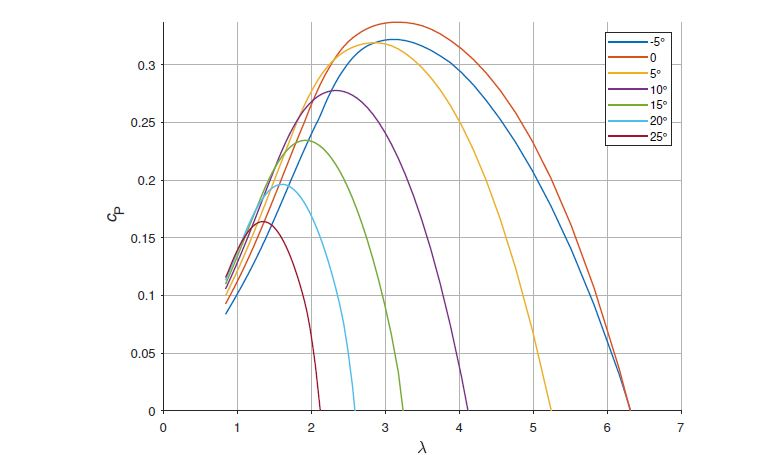
\includegraphics[width=1\textwidth]{Abbildungen/cpzulambda.jpg}
    \caption{Berechnete Leistungsbeiwerte $c_P$ des Rotors der Labor-Windkraftanlage in Abhängigkeit der Schnelllaufzahl $\lambda$ für unterschiedliche Blatt (Pitch-)Winkel.\cite{Anleitung}}
    \label{fig:cpzulambda}
\end{figure}

\newpage
\subsection{Der Momentenbeiwert \texorpdfstring{$c_M$}{}}

Der Momentenbeiwert beschreibt das Betriebsverhalten des Rotors bezüglich der Drehmoment-Abgabe. Mit dessen Hilfe lässt sich eine Aussage über das Anlaufverhalten aus dem Stillstand treffen. Dabei ergibt er sich aus dem Verhältnis des abgegebenen Drehmoments zum Luftkraftmoment, dass auf die Rotorfläche wirkt.

\begin{equation}
  c_{M}= \frac{M}{ \frac{\rho_{Luft}}{2}\cdot \pi \cdot \frac{d^3_{Rotor}}{8} \cdot v^2_{Wind} }
    \label{eq:Momentenbeiwert_cm}
\end{equation}

Des Weiteren gilt der Zusammenhang:

\begin{equation}
  c_{M}= c_{p} \cdot \lambda
    \label{eq:Momentenbeiwert_cm2}
\end{equation}

Bei Schnellläufern ist der Momentenbeiwert im Anlauf sehr gering. Dies ist Bauartspezifisch bei Schnellläufern und in Abbildung \ref{fig:cmzulambda} zu sehen.

\begin{figure}[H]
    \centering
    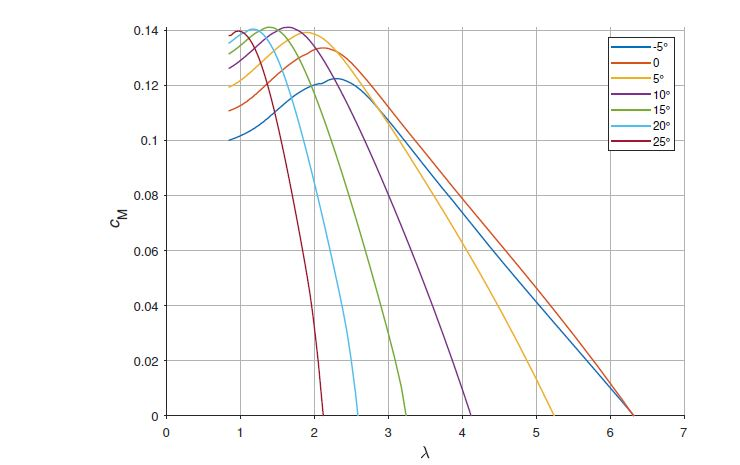
\includegraphics[width=1\textwidth]{Abbildungen/cm.jpg}
    \caption{Berechnete Momentenbeiwert $c_{M}$ des Rotors der Labor-Windkraftanlage in Abhängigkeit der Schnelllaufzahl $\lambda$ für unterschiedliche Blatt (Pitch-)Winkel.\cite{Anleitung} }
    \label{fig:cmzulambda}
\end{figure}
\newpage
\subsection{Der Schubbeiwert \texorpdfstring{$c_S$}{}}

Der Schubbeiwert $c_{s}$ ist sehr wichtig um die Windkraftanlage Struktur-mechanisch zu dimensionieren.  Dabei ergibt der Schubbeiwert aus der dynamischen Staukraft auf die Rotorfläche.

\begin{equation}
  c_{s}= \frac{F_{S}}{\frac{\rho_{Luft}}{2}\cdot \pi \cdot \frac{d^2_{Rotor}}{4} \cdot v^2_{Wind}}
    \label{eq:Schubbeiwert_cs}
\end{equation}

Der Schubbeiwert hat sein Minimum im Stillstand und sein Maximum im Leerlauf. Hier entspricht der Widerstandsbeiwert etwa dem einer Scheibe. Höhere Schubbeiwerte bedeuten, dass sie die Windkraftanlage im Propelerbetrieb befindet.\cite{Anleitung}

\begin{figure}[H]
    \centering
    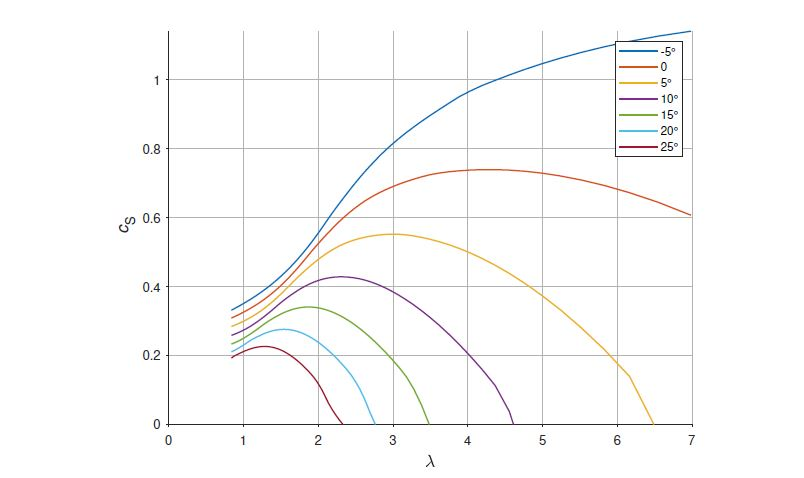
\includegraphics[width=1\textwidth]{Abbildungen/cszulambda.jpg}
    \caption{Berechneter Schubbeiwert $c_{s}$ des Rotors der Labor-Windkraftanlage in Abhängigkeit der Schnelllaufzahl $\lambda$ für unterschiedliche Blatt (Pitch-)Winkel.\cite{Anleitung}}
    \label{fig:cszulambda}
  \end{figure}

\newpage
\subsection{Verzögerung der Windgeschwindigkeit}
Wie von Betz beschrieben liegt der optimale Arbeitspunkt einer Windkraftanlage bei einem Verhältnis von $v_{1} \cdot \frac{1}{3}=v_{3}$  (Abbildung \ref{fig:Betz2905}). Dazu ist in Abbildung \ref{fig:Glauert} eine Erweiterung Glauerts zu sehen, in welcher die maximale Verblockung der Stromröhre im Leerlauf als Grenzfall berücksichtigt wird.

\begin{figure}[H]
    \centering
    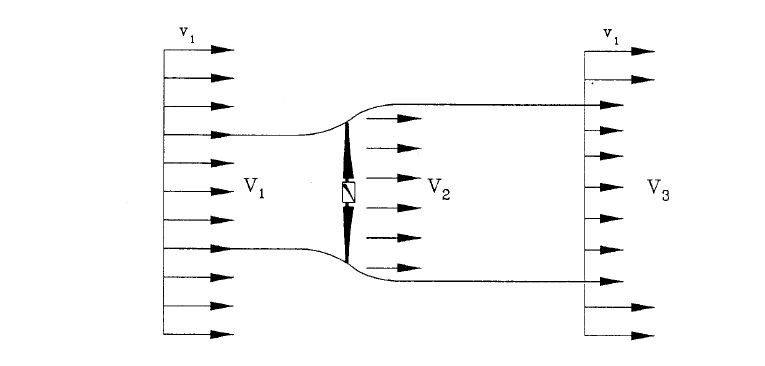
\includegraphics[width=0.9\textwidth]{Abbildungen/Betz.jpg}
    \caption{Verzögerung in der geschlossenen Stromröhre nach Betz $v_{1} \cdot \frac{1}{3}=v_{3}$ und  $v_{1} \cdot \frac{2}{3}=v_{2} $ \cite{Anleitung}}
    \label{fig:Betz2905}
\end{figure}

\begin{figure}[H]
    \centering
    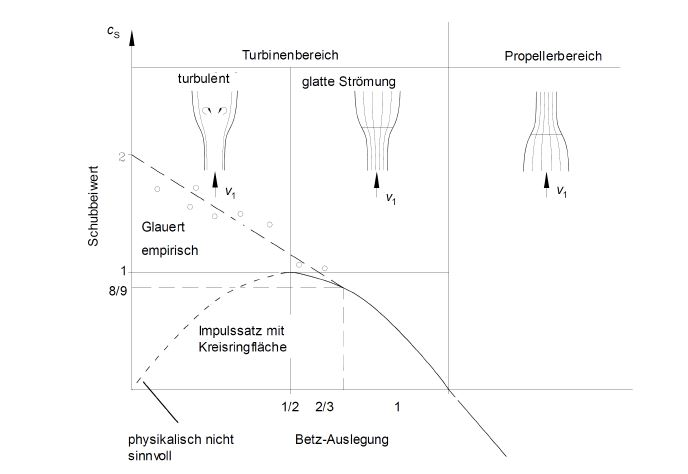
\includegraphics[width=0.9\textwidth]{Abbildungen/Glauert.jpg}
    \caption{Verzögerung in der geschlossenen Stromröhre nach Betz $v_{1} \cdot \frac{1}{3}=v_{3}$ und  $v_{1} \cdot \frac{2}{3}=v_{2} $\cite{Anleitung}}
    \label{fig:Glauert}
\end{figure}
